This chapter provides essential background information and reviews relevant prior research. It commences with an introduction to the sub-task of Question Answering (\gls{qa}), as presented in Section \ref*{sec:qa}. As previously mentioned in the Introduction (Chapter \ref{chap:intro}), this chapter maintains a clear distinction between \gls{qa} and \gls{convqa}. Consequently, Section \ref{sec:cqa} extends upon the foundational knowledge of \gls*{qa} and introduces the requisite concepts for the transformation of a QA-System into a \gls{convqa}-System. Section \ref{sec:related_work} will delve into the related work, providing a comprehensive overview of the current state-of-the-art in the field of \gls{qa} and \gls{convqa} over textual knowledge sources.

\section{Question Answering}
\label{sec:qa}

The evolution of \gls{qa} as a research field provides a solid foundation for understanding current research initiatives and methodologies. Among the early contributions is BASEBALL, an automated \gls{qa} system developed by researchers at \gls{mit} in 1961. This QA system demonstrated its capability to answer questions related to baseball using natural English language \cite{green_baseball_1961}.


In 1999, \gls{trec} (Text Retrieval Conference) initiated the \gls{trec}-8 Question Answering track, which marked "the first large-scale evaluation of domain-independent question-answering systems" \cite{voorhees_trec-8_1999}. A more well-known QA system is \textit{Watson} by IBM, an open-domain \gls{qa} system that won a the TV show Jeopardy! in 2011 \cite{ferrucci_introduction_2012}. It is evident that an evolutionary process has occurred between the early research in 1961 and today's systems like \textit{ChatGPT} by OpenAI. To understand the dimensions in which these systems differ, their components, and how to distinguish them will be introduced in Section \ref{subsec:qa_basics}, while subsequent sections will delve deeper into specific components.

In 1999, the \gls{trec} initiated the \gls{trec}-8 Question Answering track, marking \enquote{the first large-scale evaluation of domain-independent question-answering systems} \cite{voorhees_trec-8_1999}. A more renowned QA system is IBM's \textit{Watson}, an open-domain \gls{qa} system that famously triumphed on the television game show Jeopardy! in 2011 \cite{ferrucci_introduction_2012}. It is evident that an evolutionary process has transpired between the early research in 1961 and contemporary systems such as OpenAI's \textit{ChatGPT}. In section \ref{subsec:qa_basics} we will lay the groundwork by introducing the fundamental aspects of \gls{qa}-Systems and the techniques used to differentiate and categorize them. Following that, subsequent sections will delve deeper into the examination of specific system components.


\subsection{Basics}
\label{subsec:qa_basics}

Jurafsky and Martin define a \gls{qa}-System as a system \enquote{designed to satisfy human information needs} \cite{jurafsky_speech_2023}. Hence, it primarily functions as an Information Retrieval System, with its primary objective being to provide users with the desired and accurate information in response to natural language requests.

The research community has yet to establish a universally accepted classification framework for Question Answering (QA) systems. For instance, Hao et al. and Farea et al. \cite{hao_recent_2022, farea_evaluation_2022} take a comprehensive approach to classify QA systems but differ in certain aspects, such as their treatment of question types and knowledge sources. On the other hand, other researchers \cite{zhu_retrieving_2021, jurafsky_speech_2023, etezadi_state_2023, zhang_survey_2023} employ a similar classification methodology but often focus solely on retrieval-based approaches, thereby lacking a holistic perspective.

The classification proposed by Farea et al. \cite{farea_evaluation_2022} goes a step further by distinguishing between the \textbf{QA-Framework} and \textbf{QA-Paradigms}, enhancing its versatility for comparing classical and modern QA systems. An adaptation of this classification will be utilized in this thesis. The originally proposed QA algorithms have been extended to include the Retrieval-based approach, and the Question Types have been revised based on the typology introduced by Mishra et al. in their 2016 survey \cite{mishra_survey_2016}, which was further elaborated upon by Etezadi et al. \cite{etezadi_state_2023}. Also the Answer Types where adjusted to align with the classifications used in \cite{mcdonald_detect_2022,dasigi_dataset_2021}. In this context, a crucial distinction is made between a \textbf{QA} and \textbf{ConvQA} system, guided by the criteria outlined in \cite{zamani_conversational_2023}: a QA system exclusively handles standalone questions, while any inquiry exceeding a single question and involving conversational context falls within the domain of a \textbf{ConvQA} system.

The \textbf{\gls{qa}-Framework} encompasses external factors such as Question and Answer Types, while also considering system-related factors like the \gls{qa} Algorithm and Knowledge Source \cite{farea_evaluation_2022, hao_recent_2022}. Conversely, the \textbf{\gls{qa}-Paradigm} defines the fundamental underlying concept of a system and can be seen as a subset of possible combinations within the \textbf{\gls{qa} Framework}. Currently, three dominant paradigms prevail:

\begin{enumerate}
    \item \textbf{Information Retrieval (IR)-Based QA}: This paradigm involves searching through extensive multi-modal data based on a user's question and using the retrieved passages to generate an answer.
    
    \item \textbf{Knowledge Base (KB) QA}: In this approach, a semantic representation of the question is constructed, and a knowledge base is queried using this representation. The returned results are then used to generate an answer.
    
    \item \textbf{Generative Question Answering}: Here, knowledge is fully implicit, and a neural network (NN) generates answers based on its trained parameters.

\end{enumerate}

For visual clarity, a diagram illustrating the adjusted \gls{qa} Framework Classification by Farea et al. is provided in Figure \ref{fig:qa_classification}.

\begin{figure}
    \centering
    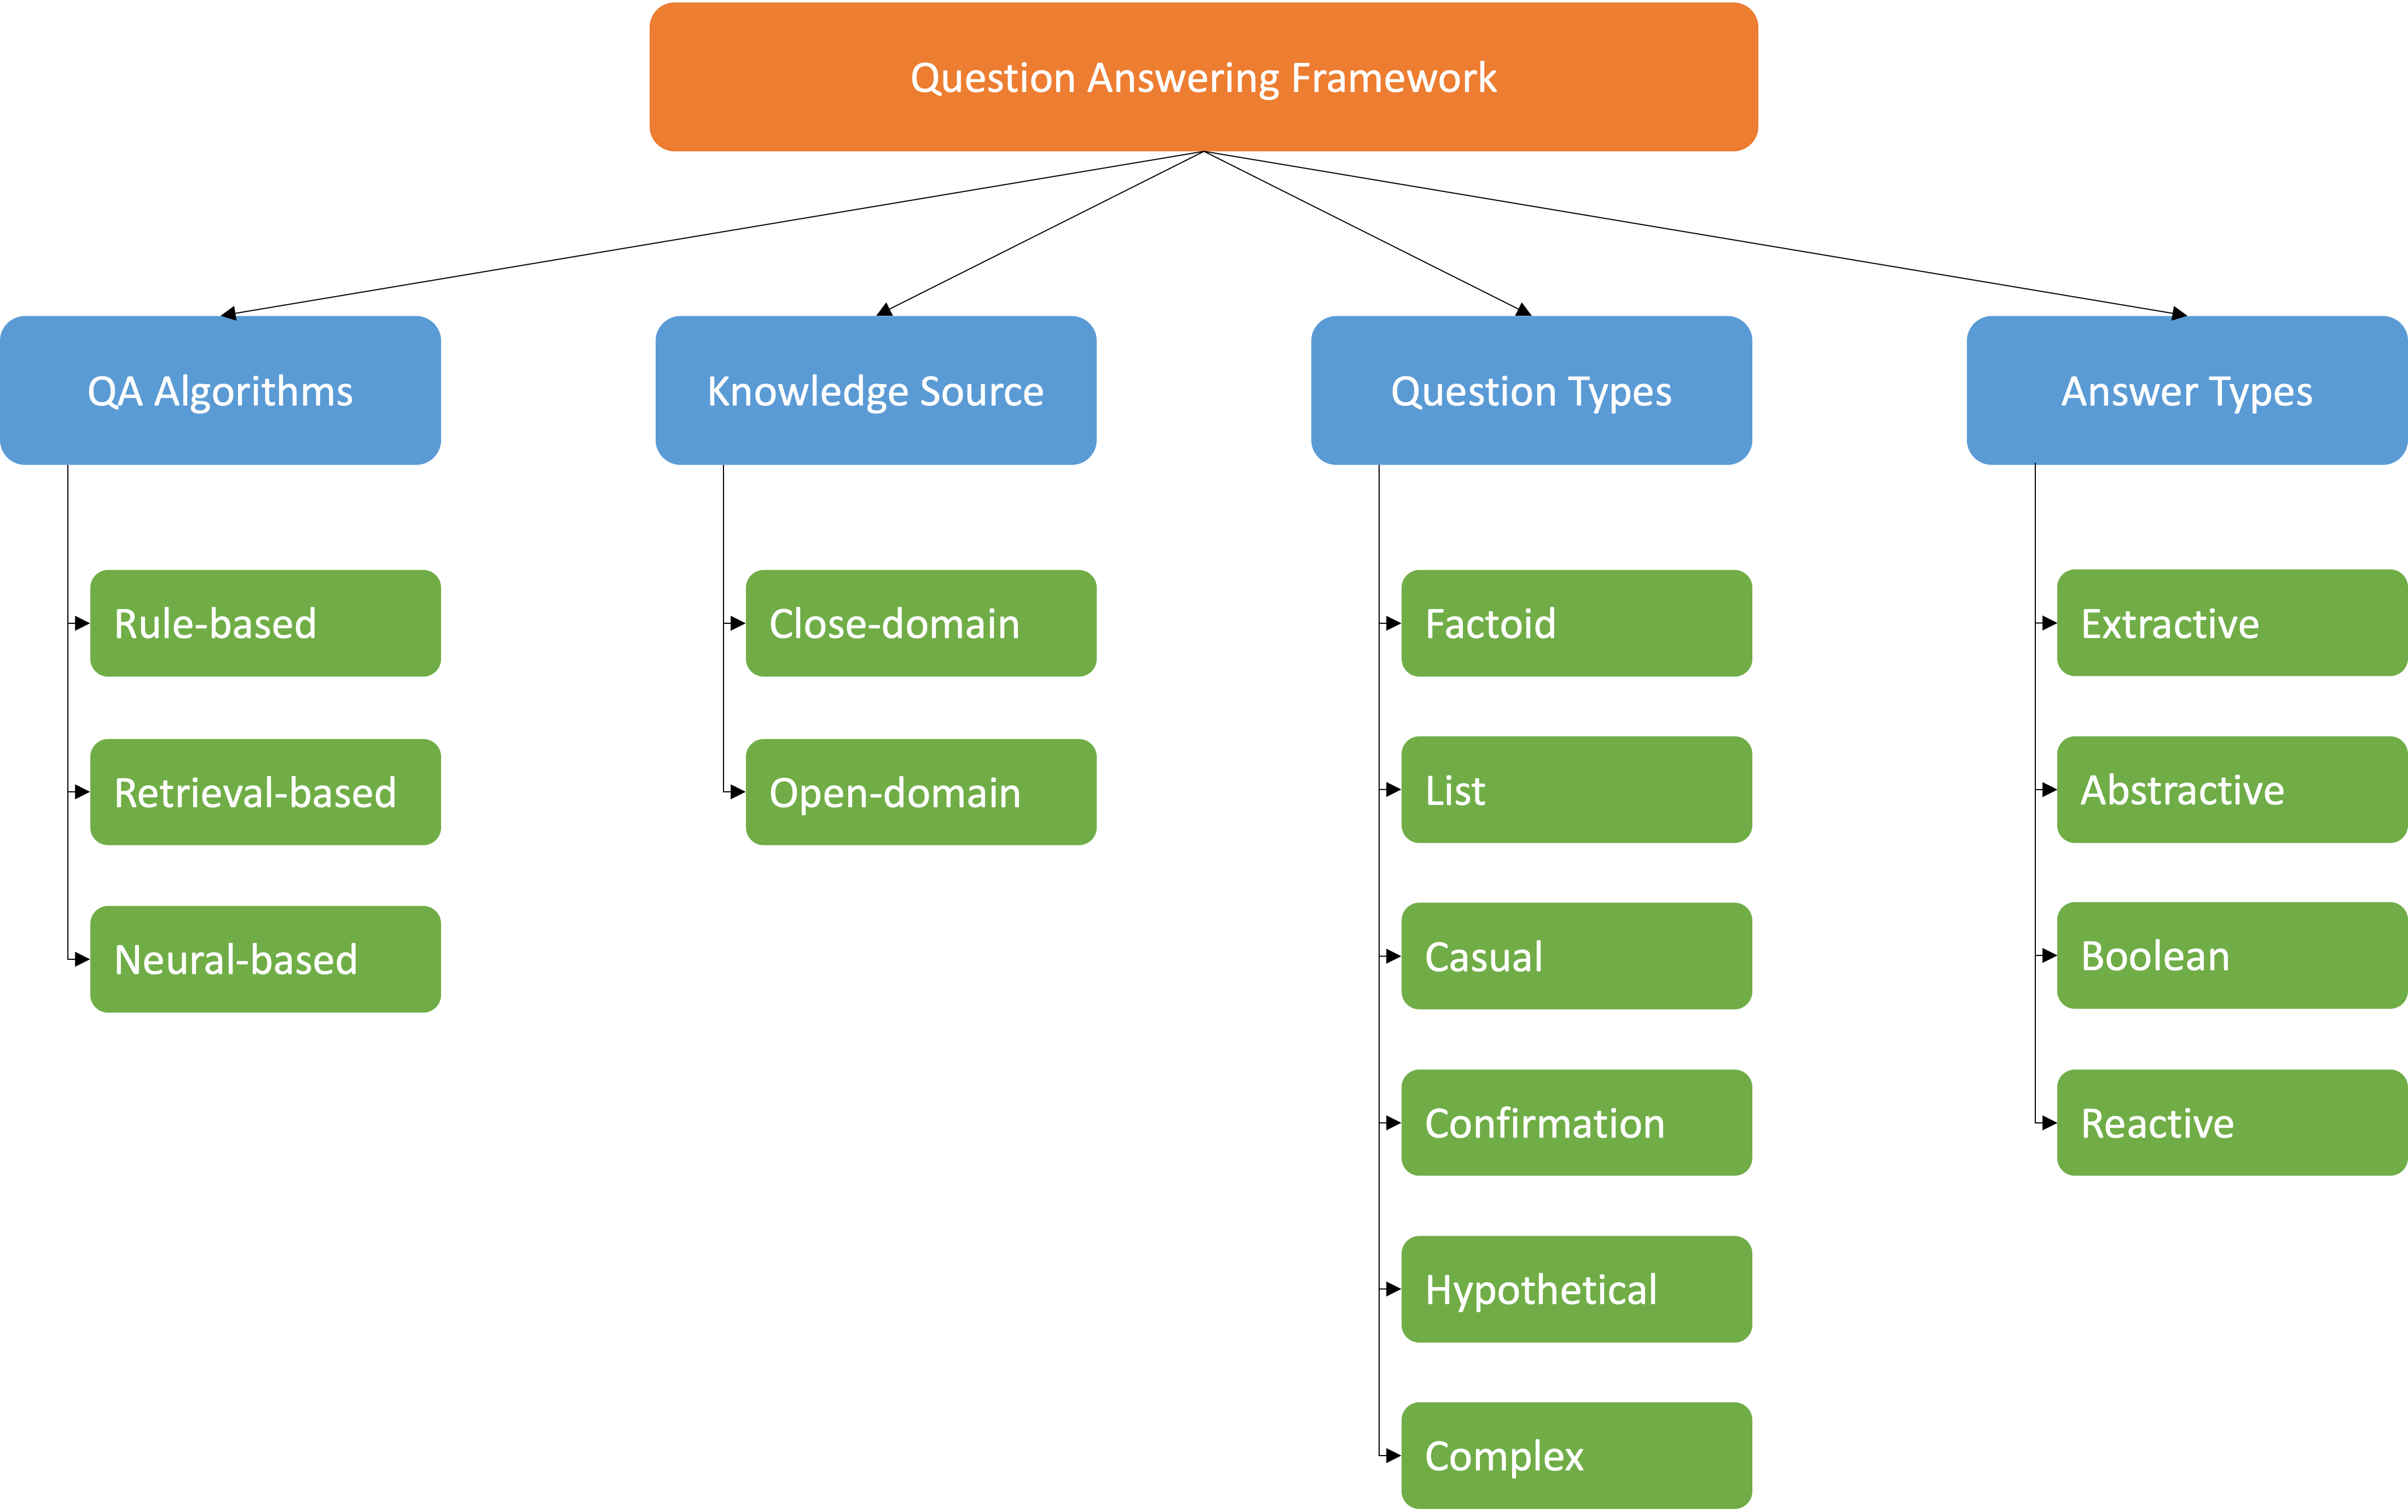
\includegraphics[width=\textwidth]{Grafiken/QA_Framework.png}
    \caption{Adjusted \gls{qa} Framework Classification by Farea et al. \cite{farea_evaluation_2022}}
    \label{fig:qa_classification}
\end{figure}


Figure \ref{fig:qa_classification} illustrates the aforementioned classification. The primary distinguishing factor is the employed \textbf{\gls{qa} Algorithm}. Rule-based approaches involve the manual crafting of feature extractions from user questions, which are then compared to the knowledge base. Rule-based approaches are typically employed in closed-domain \gls{qa} systems exclusively \cite{etezadi_state_2023}.

Retrieval-based approaches are the classic Information Retrieval (IR)-based \gls{qa} systems, comprising two key components: an intent classifier and a retriever. The intent classifier's objective is to discern the question's intent and identify important entities. Subsequently, the retriever searches the knowledge source and identifies the most relevant passages \cite{farea_evaluation_2022, zhu_retrieving_2021}.

The Neural-based approach, often referred to as the generative approach, utilizes a Sequence-to-Sequence (S2S) model to generate accurate answers to given questions. In this paradigm, the information is stored directly in the neural network's parameters, otherwise the neural network is part of a Retrieval-based approach. Most datasets in these contexts consist of triples of question, context, and answer pairs \cite{jurafsky_speech_2023}. Notably, widely used datasets such as SQuAD and QASPER originally emerged from the field of machine reading comprehension, representing a foundational step in the evolution of \gls{qa} systems \cite{rajpurkar_squad_2016, dasigi_dataset_2021, zhu_retrieving_2021}.

In addition to the \textbf{\gls{qa} Algorithms}, the \textbf{Knowledge Source} plays a pivotal role in distinguishing various aspects of Question Answering (QA) systems. The nature of the knowledge source can range from structured to unstructured or semi-structured, and it may encompass diverse data modalities, including text, audio, and video. A common point of comparison in the QA landscape is between closed and open-domain systems.

In the broad sense, a \textbf{closed-domain} QA system operates within the confines of a specific knowledge domain, which means it has limited access to information. In contrast, \textbf{open-domain} QA systems grapple with an extensive array of knowledge sources, necessitating a more versatile approach \cite{farea_evaluation_2022}.

Furthermore, a closed-domain setup often entails limitations on the types of questions it can handle, primarily focusing on factoid questions or predefined templates. Additionally, it frequently relies on structured knowledge bases like graphs or logically organized repositories \cite{hao_recent_2022}.

Conversely, open-domain QA systems are designed to tackle a wide spectrum of user queries, ranging from factoids to more complex inquiries. They typically deal with unstructured knowledge sources, which can be substantial and diverse in content \cite{zhu_retrieving_2021, farea_evaluation_2022, jurafsky_speech_2023}.

An alternative perspective for distinguishing \gls{qa}-Systems lies in the \textbf{Question Types} that users can input into the system. Questions can fall into various categories, such as \textit{factoid, list, casual, confirmation, hypothetical} \cite{mishra_survey_2016}, or \textit{complex} \cite{etezadi_state_2023}.

\begin{itemize}
   \item \textit{Factoid questions}, the most common type, are typically signaled by question words (what, when, which, who, how) and yield a concise factual answer.
   
   \item \textit{List questions} represent a specialized subset of factoid questions, where the answer comprises a list of facts.
   
   \item \textit{Casual questions} encompass inquiries that deviate from the factoid format, often involving words like \textit{how} or \textit{why} and requiring more advanced reasoning.
   
   \item \textit{Confirmation questions} seek simple yes or no responses, frequently employed in personal assistant applications.
   
   \item \textit{Hypothetical questions} delve into hypothetical scenarios (e.g., "what would happen if"), aiming for plausible rather than definitive answers.
   
   \item \textit{Complex questions} can be further categorized into \textit{answer-retrieval-complex} and \textit{question-understanding-complex}. In the case of question-understanding-complex questions, the complexity arises from nuances like multiple constraints, making the question itself intricate to comprehend. In contrast, answer-retrieval-complex questions involve complexities in finding the correct answer, often requiring the combination of information from multiple documents or similar sources. This is commonly referred to as long-form \gls{qa}.
\end{itemize}

Lastly, a \gls{qa}-System can be characterized by the \textbf{Answer Types} it offers, a concept closely intertwined with Question Types. Farea et al. \cite{farea_evaluation_2022} delineate three categories of answers: \textit{extractive, abstractive, boolean} and \textit{reactive}. 

\begin{itemize}
   \item \textit{Extractive answers} represent the most common type, where the answer is a specific factual excerpt presented as a span of tokens.

   \item \textit{Abstractive answers} typically correspond to complex questions that necessitate the system to consider multiple documents and information sources to formulate a response. In such cases, no predefined or annotated answer exists.

   \item \textit{Boolean answers} are typically the result of confirmation questions, where the answer is either \textit{yes} or \textit{no}.

   \item \textit{Reactive answers} often arise in response to confirmation questions and can be a system-generated reaction based on the user's provided answer.
\end{itemize}

% Pushed 1st

\subsection{Information Retrieval Architectures}
\label{subsec:qa_architectures}

As stated in the previous section (Section \ref{subsec:qa_basics}), there are three major paradigms in \gls{qa}: \gls{ir}-based \gls{qa}, \gls{kb}-based QA, and Generative \gls{qa}. This section will primarily concentrate on the first paradigm, \gls{ir}-based QA, as it holds the most promise for addressing the objectives of this thesis topic.

This thesis will not focus on \gls{kb} QA, as this approach requires the mapping of the query to a structured data representation. As the task of this thesis is to develop a general system, which is adaptable to different data inputs, \gls{kb} QA will be excluded \cite{dimitrakis_survey_2020}.

Generative \gls{qa} is often denoted as \textit{Retriever-free} or \textit{Neural-based} approaches. The central characteristic of this paradigm is that knowledge resides within the parameters of a neural network. Consequently, the knowledge is implicit, and the \gls{qa} system will not furnish a specific document, passage, or other source from which it extracted the information. Instead, it offers a textual excerpt. While these systems can achieve competitive performance compared to \gls{ir}-based \gls{qa} systems, they are not under consideration for this thesis due to their lack of reference, which is a crucial requirement for the system to be developed \cite{roberts_how_2020}.


\begin{figure}
    \centering
    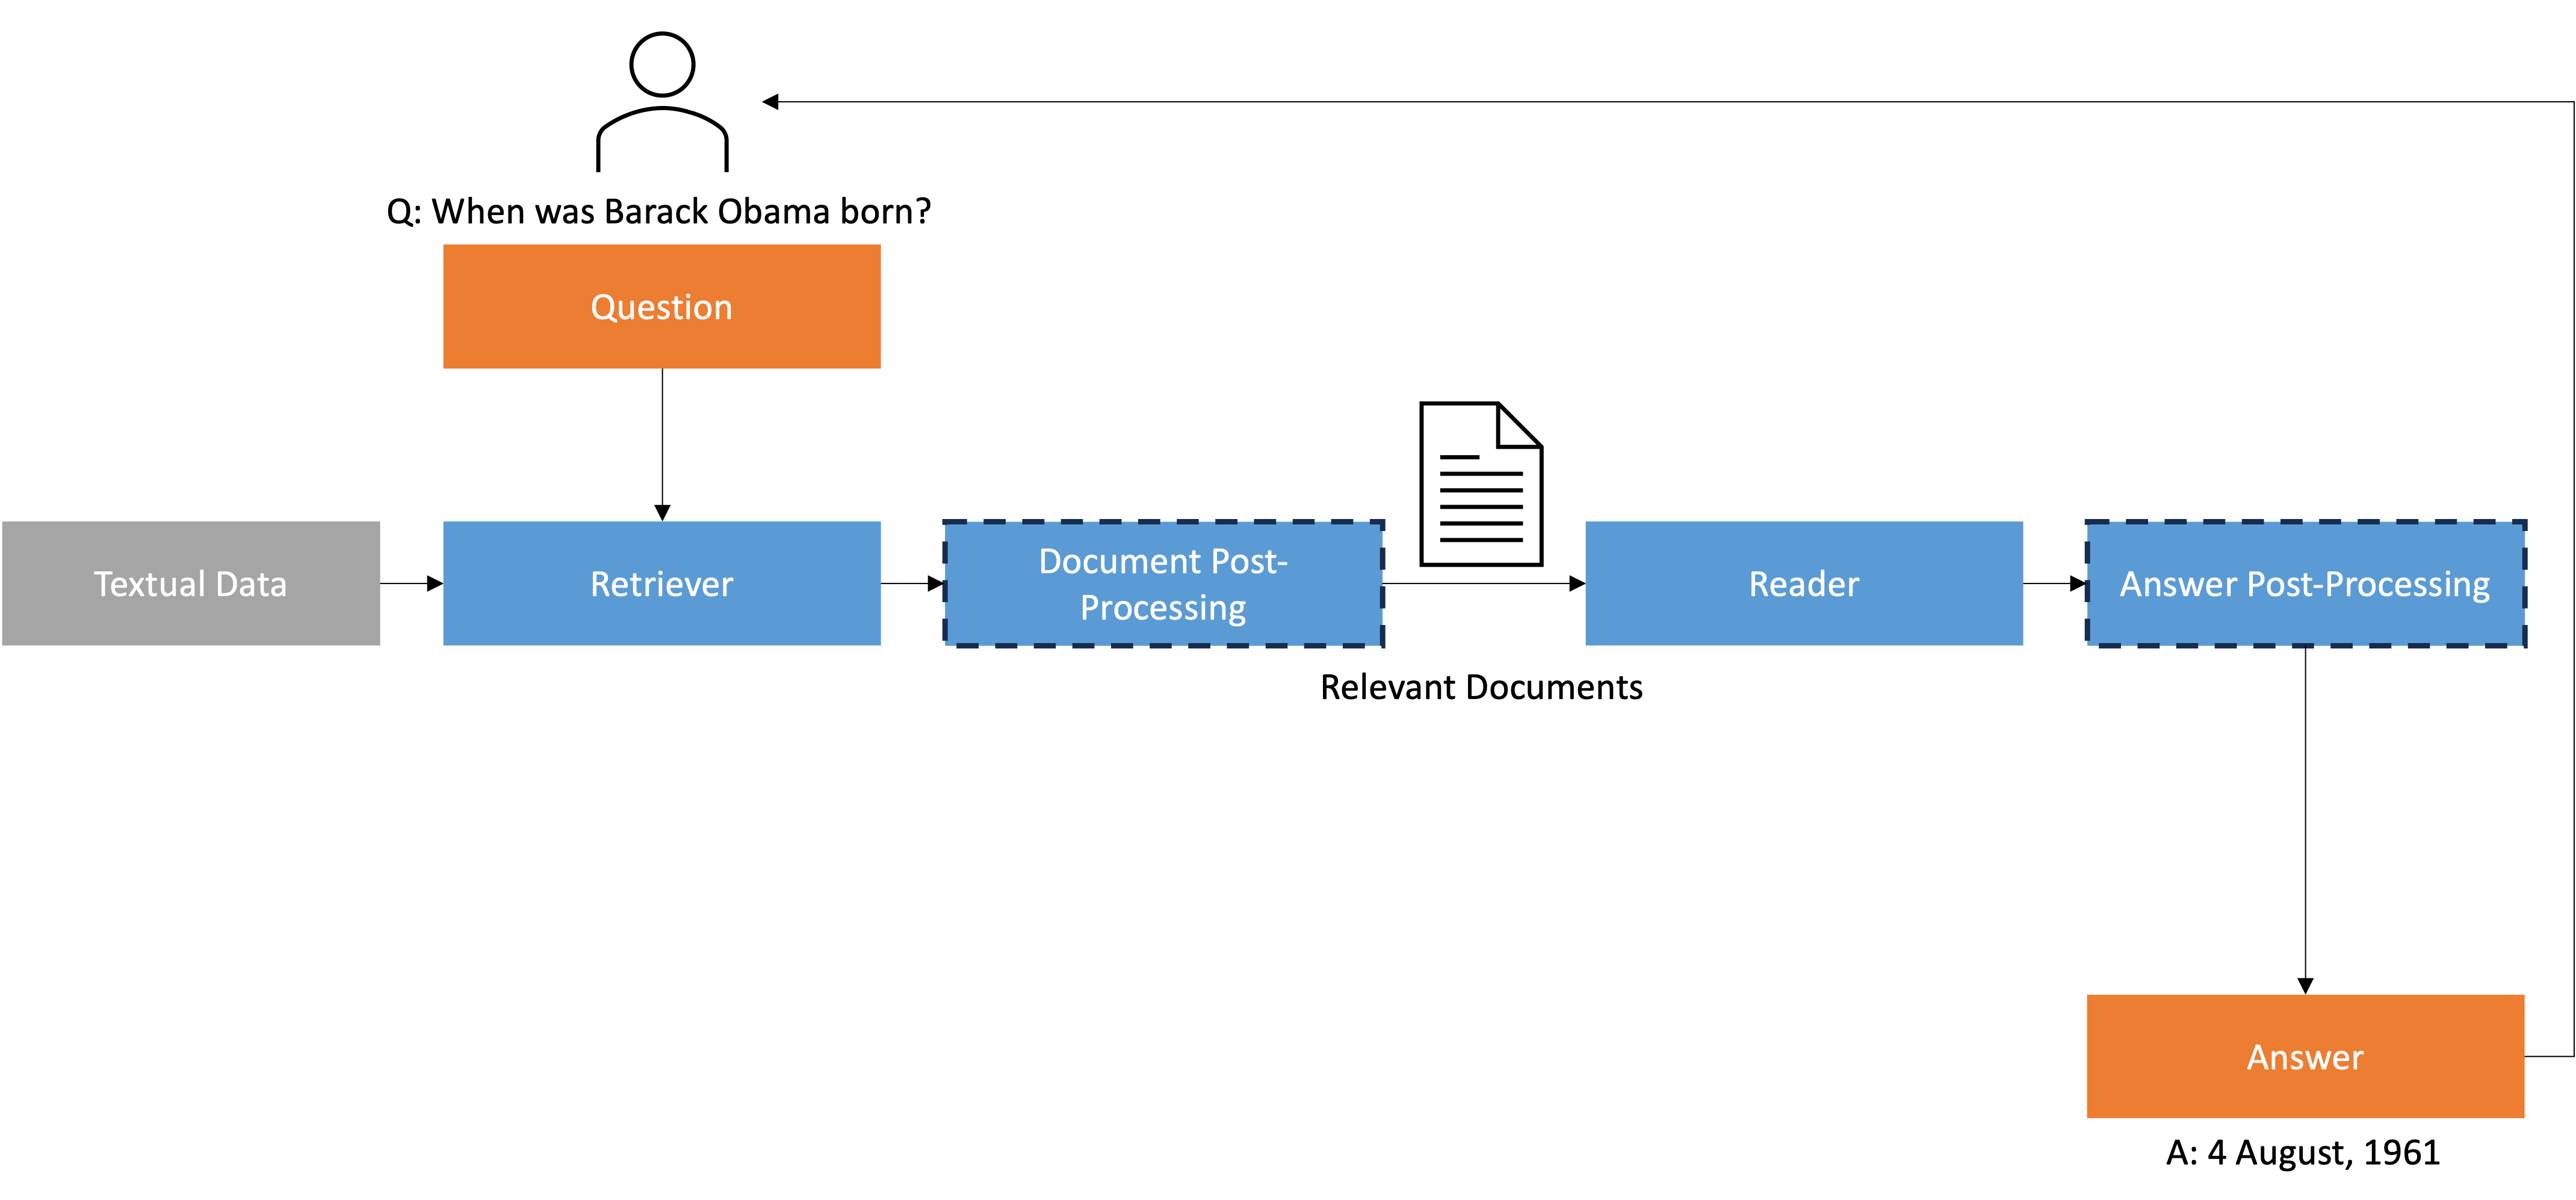
\includegraphics[width=\textwidth]{Grafiken/Retriever_Reader.png}
    \caption{Reader-Retriever-System Architecture for \gls{qa} by Zhu et. al. \cite{zhu_retrieving_2021}. The dashed lines indicate optional modules.}
    \label{fig:rr_architecture}
\end{figure}

Figure \ref{fig:rr_architecture} depicts the general architecture of a \textbf{Retriever-Reader-System}, as defined by Zhu et al. \cite{zhu_retrieving_2021}. This architecture serves as the foundational framework for \gls{ir}-Based \gls{qa} systems and was initially introduced by Harabagiu et al. \cite{harabagiu_open_domain_2003}. In this framework, all modules operate independently, can be trained separately, and are subject to independent evaluation.

The \textbf{Retriever} module's primary role is to retrieve relevant documents, passages, or other pertinent information from a knowledge source and rank them based on their relevance to answering the user's query. Subsequently, the \textbf{Reader} module extracts the answer from the retrieved documents and presents it to the user. This task bears a close resemblance to \gls{mrc}, with the key distinction that in \gls{ir}-Based \gls{qa}, the system must handle multiple documents and comprehend them to formulate a response, unlike classical \gls{mrc} tasks, which typically involve only one context document.

The \textbf{Document Post-Processor} module's role is to curate and refine the set of documents that will be forwarded as "Relevant Documents" to the subsequent stage, the Reader. Concurrently, the \textbf{Answer Post-Processor} assists the Reader in addressing complex questions for which the answer may not be found in a single document alone \cite{zhu_retrieving_2021,jurafsky_speech_2023}.

It's worth noting that some researchers include a \textbf{Question Analysis} module preceding the Retriever, which aims to preprocess the received question for more efficient query execution in the Retriever \cite{nassiri_transformer_2023}. However, for the purposes of this thesis, we adhere to Zhu et al.'s definition \cite{zhu_retrieving_2021}, where this functionality is considered part of the Retriever.

Conceptually, there are three distinct approaches to the Retriever itself: \textit{Sparse Retrieval, Dense Retrieval,} and \textit{Iterative Retrieval.} The specifics of these approaches will be thoroughly explored in Section \ref{subsec:qa_retrieval}.

Document Post-Processors can be categorized into \textit{Supervised Learning, Reinforcement Learning,} and \textit{Transfer Learning}-based approaches. A detailed discussion of these approaches is also provided in Section \ref{subsec:qa_retrieval}.

In Section \ref{subsec:qa_user_interaction}, we will delve into the finer details of Reader approaches and Answer Post-processing. Broadly speaking, there are two primary types of Readers: \textit{Extractive} and \textit{Generative} Readers. As for Answer Post-processing, it involves two key categories: \textit{Rule-based} and \textit{Learning-based} approaches.

There are also \textbf{End-to-End} approaches that employ a single module to execute the entire \gls{qa} task. Excluding generative approaches, two common categories of such approaches are \textbf{Retriever-Reader} and \textbf{Retriever-only} models.

An End-to-End Retriever-Reader aims to train both the Retriever and Reader in a single backpropagation step, and in some cases, it introduces additional knowledge sources beyond the traditional \gls{ir} framework. An illustrative example is \gls{rag} \cite{lewis_retrieval-augmented_2021}. \gls{rag} consists of a pre-trained Generator with implicit knowledge encoded in its parameters and a pre-trained Retriever. For each question, the Retriever identifies the most relevant documents and generates a latent vector based on them. This latent vector, along with the original question, is fed into the Generator.

Another end-to-end approach, similar to \gls{rag}, is \gls{realm} \cite{guu_realm_2020}. While these previous two approaches extended the capabilities of pre-trained \gls{s2s} models, Nishida et al. pursued a different path by training a single \gls{nn} to perform both tasks simultaneously: \gls{ir} and \gls{mrc} \cite{nishida_retrieve-and-read_2018}.

It is noteworthy that all these end-to-end approaches have demonstrated competitive performance compared to state-of-the-art methods on specific \gls{qa} datasets.

An essential yet often underestimated question is: What defines textual data, and how should one preprocess formats such as PDFs to extract this textual content? While many datasets already comprise small contextual snippets \cite{wang_modern_2022}, it's crucial not to overlook the entire process of extracting snippets from unstructured PDFs, for example. Approaches to tackle this challenge will be explored in detail in the upcomming Section \ref{subsec:qa_indexing}.

% 2nd push

\subsection{Extraction Approaches}
\label{subsec:qa_indexing}

As discussed in the previous Section \ref{subsec:qa_basics}, the knowledge source for a \gls{qa}-System can take the form of textual or multimodal data. The specific type of data may necessitate certain requirements or specific adjustments to the Retriever used for \gls{ir}.

In the context of this thesis, the primary knowledge source to be employed is PDF documents. In the research field, three major approaches exist for extracting textual information from unstructured data types like PDFs: \textit{visual} \cite{tito_document_2021}, \textit{direct} \cite{wang_multi-passage_2019}, and \textit{alternative} \cite{dasigi_dataset_2021} extraction methods.

It's important to note upfront that the chosen extraction method is intricately connected to the subsequent retrieval approach. The specifics, including metadata alongside pure textual data and quality requirements, may vary among different extraction and retrieval methods.

The visual approach is closely aligned with the research field of \textit{Document Question Answering}. A well-known example dataset in this field is \gls{docvqa} \cite{tito_document_2021}. The primary concept behind the visual approach to document question answering is to capture not only the text of a PDF but also additional information such as the document's structure, various hierarchies on a page (e.g., sections, subsections), and the ability to analyze tables and figures. These hierarchical structures can be leveraged to create two-stage retrieval approaches. In these approaches, initially, a collection of relevant files is identified based on higher-level attributes like the document's title and abstract. Subsequently, a more granular retrieval process is executed over lower-level attributes such as passages within the relevant files. These \textit{Iterative Retrievers} will be further discussed in Section \ref{subsec:qa_retrieval} \cite{liu_dense_2021}.

The challenge of \textit{Visual Document Question Answering} typically involves taking images of PDF pages as inputs and mapping question-answer pairs to them. The answers are extracted from either a single paragraph or a combination of multiple paragraphs \cite{mathew_document_2021}. Nonetheless, the extraction pipeline in this case usually resembles the \textit{Retriever-Reader} architecture, where the extracted information from the visual processing is fed into such a system afterward. Researchers in this field often employ a pipeline that includes a \textit{Document Layout Analysis} model, followed by the application of an \gls{ocr} tool to the detected regions \cite{mcdonald_detect_2022}. Examples of a \textit{Document Layout Analysis} model include the Document Image Transformer by Li et al. \cite{li_dit_2022}.

The direct approach is the most prevalent method in the field of Question Answering (\gls{qa}) and Information Retrieval (\gls{ir}). The primary concept behind this approach is to extract textual information from PDFs and store it in a database. The extraction process can be accomplished using various tools such as \textit{PDFMiner} or \textit{Adobe Extract} \cite{meuschke_benchmark_2023}. However, a lingering question is how to effectively split the extracted textual data, especially considering that they are often not cleaned after extraction.

A common practice when employing a Language Model (\gls{llm}) is to optionally cleanse the text corpus and then divide it based on a predefined token size. This approach is evident in two notable open-source LLM projects: \textit{Langchain} and the \textit{Retrieval Plugin for ChatGPT} by OpenAI \cite{noauthor_langchain-ailangchain_nodate,noauthor_chatgpt_2023}. In the original Dense Retrieval paper by Karpukhin et al., a sliding window of token size 5 was utilized \cite{karpukhin_dense_2020}. Therefore, it can be assumed that for contemporary LLM applications, the precise quality of the data, ensuring that a document contains syntactically correct sentences, may not be as critical.

Apart from modern approaches involving text clipping, previous methods aimed to identify paragraphs and similar structures within the extracted texts \cite{zhu_retrieving_2021}.

An alternative approach involves the methodology employed in constructing the QASPER dataset. In this case, the authors conducted a pre-filtering of scientific papers' PDFs, selecting only those with freely accessible LaTeX files. They then utilized the S2ORC tool to extract cleaned textual data from these LaTeX files \cite{dasigi_dataset_2021}. It's important to note that this approach is highly specific to the QASPER dataset and cannot be universally applied. Nonetheless, it serves as an illustration of alternative methods for extracting textual data from PDFs.

% Commit #3

\subsection{Retrieval Approaches}
\label{subsec:qa_retrieval}

The traditional state-of-the-art in \gls{ir} relies on \textbf{Sparse Retrievers}, with one notable example being BM25. BM25 is renowned as "one of the most empirically successful retrieval models and is widely used in current search engines" \cite{zhu_retrieving_2021}. Nandan et al. even demonstrated that on modern \gls{odqa} datasets, BM25 remains a viable baseline for zero-shot \gls{ir} \cite{thakur_beir_2021}.

BM25 was originally introduced by Robertson et al. \cite{robertson_probabilistic_2009}. It operates by utilizing the TF-IDF token weights between a question $q$ containing tokens $q_1, \ldots, q_T$ and a set of passages $P$, where $p \in P$.

\begin{equation}
    \mathbf{s}_{q, p}^{\text{BM25}}=\sum_{i=1}^T \log \left(\frac{|\mathcal{P}|}{N\left(q_i, \mathcal{P}\right)}\right) \frac{n\left(q_i, p\right)\left(k_1+1\right)}{k_1\left(1-b+\frac{b|p|}{a v p l}\right)+n\left(q_i, p\right)}
    \label{eq:bm25}
\end{equation}

    
Equation \ref{eq:bm25} illustrates the BM25 score for a question $q$ and a passage $p$. In this equation, $N\left(q_i, \mathcal{P}\right)$ represents the count of passages in $\mathcal{P}$ that contain the token $q_i$, while $n\left(q_i, p\right)$ indicates the frequency of token $q_i$ within the passage $p$. The variable $|p|$ signifies the length of passage $p$, and $avpl$ stands for the average passage length in $\mathcal{P}$. The parameters $k_1$ and $b$ are free parameters, typically set to $k_1 = 0.9$ and $b = 0.4$ \cite{mcdonald_detect_2022,robertson_probabilistic_2009}.

Traditionally, this lexical Information Retrieval (\gls{ir}) approach has been capable of providing satisfactory retrieval results. However, in 2020, Karpukhin et al. demonstrated for the first time that a \textbf{Dense Retrieval} approach could outperform the Sparse Retrieval approach across multiple \gls{odqa} datasets \cite{karpukhin_dense_2020}. Consequently, the search for a general Dense Retrieval model has been ongoing, as these Dense Retrieval approaches offer advantages such as semantic matching and the ability to handle lengthy documents \cite{zhu_retrieving_2021}.

In general, there are three types of Dense Retrieval approaches \cite{zhu_retrieving_2021}: the \textbf{Representation-based Retriever}, often referred to as the \textit{dual-encoder} \cite{karpukhin_dense_2020}; the \textbf{Interaction-based Retriever}, often referred to as the \textit{cross-encoder}; and the \textbf{Representation-interaction Retriever}, often referred to as the \textit{multi-stop retriever}. Figure \ref{fig:types_of_retriever} illustrates the general architecture of these three types of Dense Retrievers.

The \textbf{Dense Passage Retriever (DPR)} by Karpukhin et al. serves as a notable example to explain the \textbf{Representation-Based Retriever}. Given a collection $M$ of text passages $p$ and a question $q$, the objective of DPR is to identify the $k$ most similar passages to the question. To achieve this, DPR employs two distinct \textbf{BERT} \cite{devlin_bert_2019} Encoders. One Encoder, denoted as $E_Q(\cdot)$, encodes the question $q$ into a $d$-dimensional vector, where $d = 768$. The other Encoder, labeled as $E_P(\cdot)$, encodes the passage $p$ into a $d$-dimensional vector at the \verb|[CLS]| token. The similarity between these two vectors is computed using the inner product:


\begin{equation}
    \mathbf{s}_{q, p}^{D P R}=\mathbf{E}_{Q}(q)^{\top} \mathbf{E}_{P}(p)
    \label{eq:dpr}
\end{equation}

The choice of the inner product as the similarity function is motivated by its computational efficiency and the demonstrated, comparable performance \cite{karpukhin_dense_2020}. It is crucial for the dot-product to yield a small value for pairs of questions and passages that are genuinely related. The training dataset $D$ comprises $m$ instances, where $q_i$ represents the question, $p_i^+$ denotes the positive passage, and $p_{i,n^-}$ represents the negative passage:

\begin{equation}
    \mathbf{D}=\left\{\left(q_{i}, p_{i}^{+}, p_{i, 1}^{-}, \ldots, p_{i, n}^{-}\right)\right\}_{i=1}^{m}
\end{equation}

The loss function is optimized using the negative log likelihood of $p_i^+$:

\begin{equation}
    \mathcal{L}_{D P R}=-\log \frac{\exp \left(\mathbf{s}_{q_i,p_i^{+}}^{D P R}\right)}{\exp \left(\mathbf{s}_{q_i,p_i^{+}}^{D P R}\right) + \sum_{j=1}^{n} \exp \left(\mathbf{s}_{q_i,p_{i,j}^{-}}^{D P R}\right)}
\end{equation}

It's important to note that in \cite{karpukhin_dense_2020}, the selection of negative passages was not arbitrary. Instead, two additional approaches were employed: BM25 top passages that do not contain the answer and positive passages paired with other questions.

One significant advantage of the Representation-Based Retriever is that passages can be pre-indexed locally rather than at runtime. This reduction in latency between the question and the response may, however, come with trade-offs in the quality of the retrieved passages.

The \textbf{Interaction-Based Retriever} incorporates both the question $q$ and the passage $p$ within a single model, separated by a \verb|[SEP]| indicator. These models offer various approaches for modeling the relationship between $q$ and $p$. For instance, one common method is to utilize the \verb|[CLS]| classifier as an indicator of whether the passage is relevant to the question. This approach was first introduced with \gls{bert} \cite{devlin_bert_2019}. While these models perform competitively with previous Representation-Based Retrievers, it's important to note that they are 100-1000 times more computationally expensive \cite{khattab_colbert_2020}.

To address this latency issue, models like ColBERT introduced the concept of \textbf{co}ntextualized \textbf{l}ate ineraction \cite{khattab_colbert_2020}. In this thesis and subsequently in research, it is referred to as the \textbf{Representation-Interaction Retriever} \cite{zhu_retrieving_2021}.


\begin{figure}
    \centering
    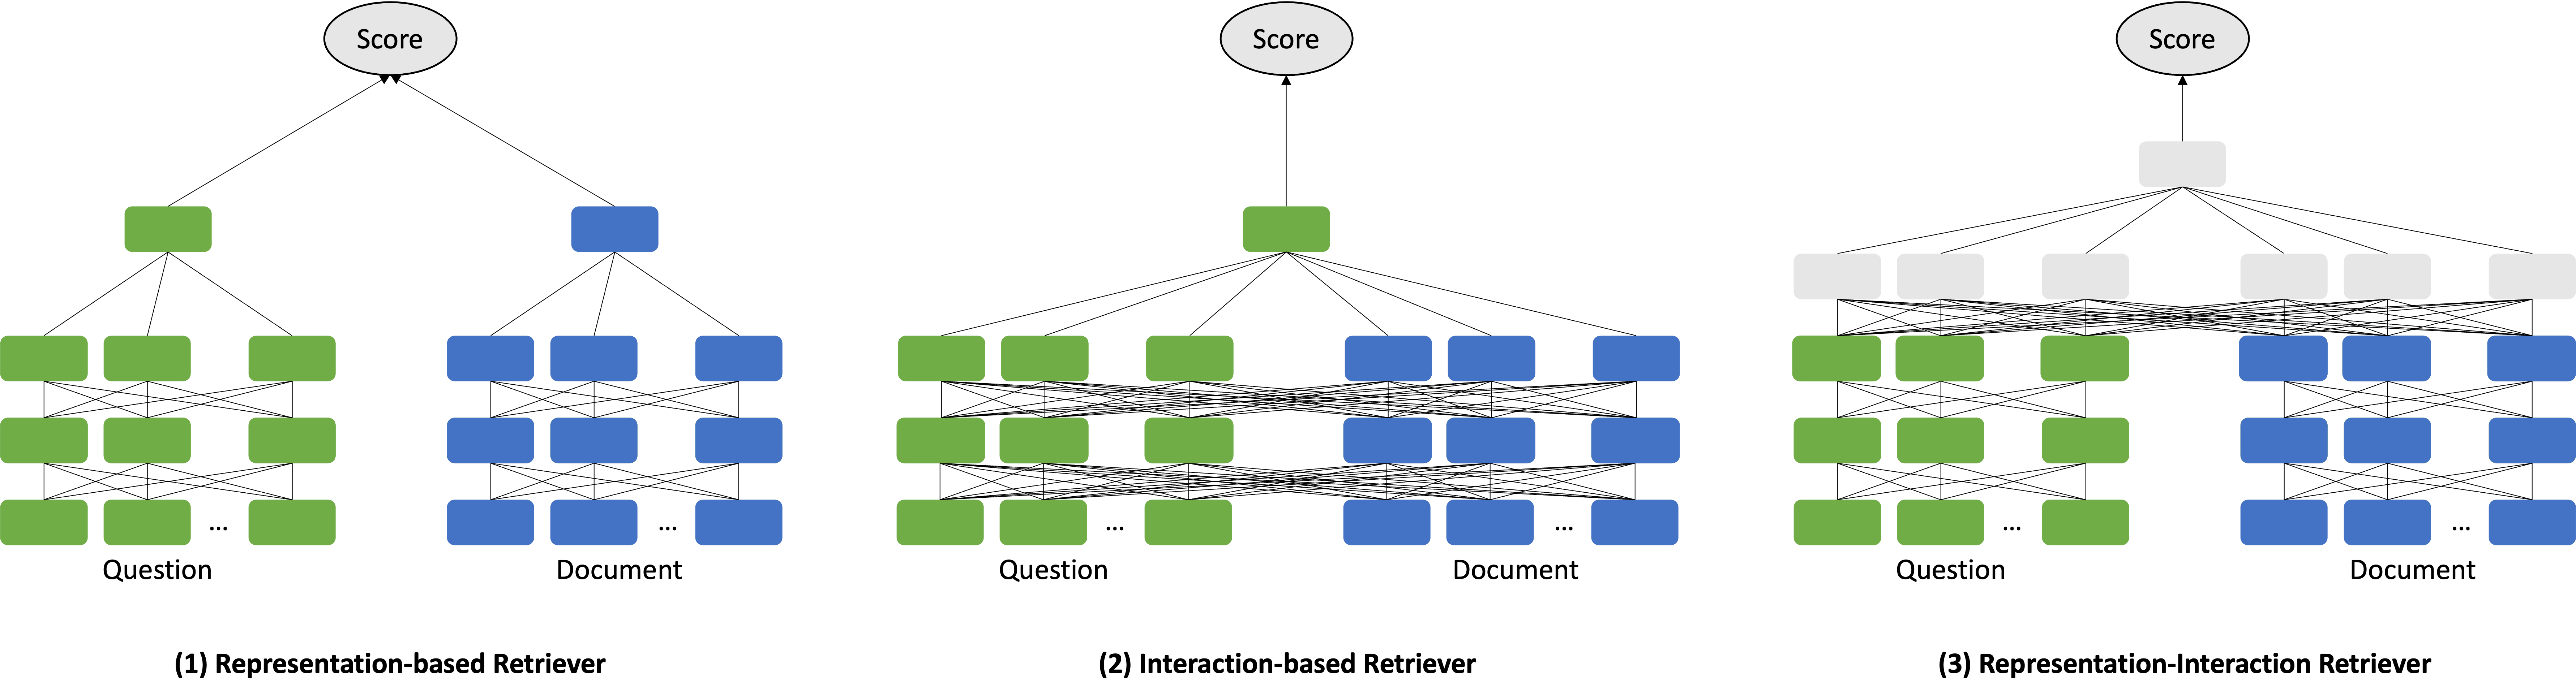
\includegraphics[width=\textwidth]{Grafiken/Types_of_Retriever.png}
    \caption{Types of Dense Retriever by Zhu et. al. \cite{zhu_retrieving_2021}.}
    \label{fig:types_of_retriever}
\end{figure}

ColBERT, like \gls{dpr}, employs two \gls{bert} Encoders, denoted as $E_Q\left(\cdot\right)$ and $E_P\left(\cdot\right)$. However, it introduces a late interaction mechanism. When provided with a query $q$, it is initially tokenized into BERT-based Wordpiece tokens, resulting in $q_1, \ldots, q_T$. Following the \verb|[CLS]| token, a \verb|[Q]| token is appended to signify the question. If the length of the tokenized question is less than $N_q$, a predetermined token length, the remaining portion of the question is padded with BERT's \verb|[mask]| token. Otherwise, it is truncated. This process, known as *query augmentation*, allows BERT to re-weight existing terms or expand the query, and it is pivotal to ColBERT's performance. The generated embeddings are then passed through a linear layer to reduce the output dimensions to a fixed size $m$, which is smaller than the original dimensions of BERT. The output is subsequently normalized to ensure that the L2 norm of each result equals one.

For each passage $p$, $E_P\left(\cdot\right)$ is employed for encoding. Similar to the question encoding process, $p$ is segmented into its $p_1, \ldots, p_{T_d}$ Wordpiece tokens. The special token \verb|[D]| indicates a passage. Short passages are not padded with a \verb|[mask]| token. After the classical BERT output, a similar post-processing step is applied to the encoded passages, and all embeddings corresponding to punctuation are filtered out.

\begin{equation}
    \mathbf{E}_{q}:= Normalize(CNN(BERT("[Q] q_0 q_1 \dots q_T [mask] \dots [mask]")))
\end{equation}

\begin{equation}
    \mathbf{E}_{p}:= Filter(Normalize(CNN(BERT("[D]p_0 p_1 \dots p_T"))))
\end{equation}

The late interaction mechanism applied to the encodings involves computing the maximum similarity, which utilizes cosine similarity through dot-products. This is made possible by the earlier normalization applied to the embeddings:

\begin{equation}
    \mathbf{s}_{q, p}^{C o l B E R T}=\sum_{I\in\left[\left|\mathbf{E}_q\right|\right]}\max _{j\in\left[\left|\mathbf{E}_d\right|\right]} \mathbf{E}_{q, i} \cdot \mathbf{E}_{p, j}^{\top}
\end{equation}

The interaction mechanism has no trainable parameters. ColBERT is differentiable end-to-end. During training, for example, with a triple $(q, p^+, p^-)$, ColBERT independently produces a score for each passage and is subsequently optimized pairwise using softmax cross-entropy loss over the scores of $p^+$ and $p^-$ \cite{khattab_colbert_2020}.

Another type of Retriever is the \textbf{Iterative Retriever}. Iterative Retrievers are necessary when dealing with questions that are more complex than simple factoid questions, which can be answered by identifying the right passage in the knowledge source. An example is the HotpotQA dataset \cite{yang_hotpotqa_2018}, designed specifically for multi-hop questions. The fundamental concept here is that such questions cannot be answered with just one precise piece of evidence. They require multiple passages from different documents at the very least. Iterative Retrievers encompass three stages in the pipeline: (1) document retrieval, (2) query reformulation, and (3) retrieval stopping.

An example is BEAM, currently holding the title of the highest-performing\footnote{Status as of September 23, 2023, according to https://paperswithcode.com and the authors of \cite{zhang_beam_2023}}, \gls{qa}-System across multi-hop \gls{qa} datasets such as HotpotQA \cite{zhang_beam_2023}. The document retrieval component can take the form of any retrieval model, including options like ColBERT, BM25, or \gls{dpr}. In the case of BEAM, it leverages an Interaction-Based Retriever using DeBERTa. For each candidate passage $p_c$, BEAM calculates a relevance score concerning this passage within the context of all previously identified relevant passages $p_r$ and the question $q$, using the embeddings of the \verb|[CLS]| tokens \cite{he_deberta_2020}. The second step, query reformulation, can be executed explicitly or implicitly, meaning it can either be expressed in natural language or as a dense embedding. The advantage of using natural language lies in its interpretability, while employing dense embeddings operates within a semantic space and does not lack vocabulary interpretability \cite{zhu_retrieving_2021}. BEAM adopts a natural language-based approach. Specifically, after each hop, it appends the newly identified passage to the previously identified ones and feeds this information into DeBERTa.

\begin{equation}
    \text{s}_{q, p}^{BEAM} = \text{Classifier}(\text{DeBERTa}("[CLS] q \: p_{r_1} \: \ldots \: p_{r_i} \: ")) \quad | \quad p_{c} \in P
\end{equation}

The nature of query reformulation depends on the type of retriever in use. Lastly retrieval stopping poses its own set of challenges. A common approach involves setting either a fixed number of hops or a maximum limit on the retrieved documents. Alternatively, some methods introduce a new token, such as \verb|[EOE]| (End-of-Evidence), to signal the end of retrieval \cite{zhu_retrieving_2021}. BEAM, for example, employs a fixed number of hops, specifically 2, as determined through empirical evaluation.

The task of \textbf{Document Post-Processing} is to reduce the number of passages forwarded to the Reader, aiming to eliminate irrelevant ones. Traditional Retrievers, like Sparse Retrievers, often required a Document Post-Processor. However, Dense Retrievers often incorporate ranking and retrieval simultaneously, rendering this module unnecessary \cite{zhu_retrieving_2021}. Nevertheless, it remains possible to construct multi-stage Retrievers to, for instance, increase latency. This can be achieved by using a simpler Dense Retriever for pre-filtering passages and subsequently applying a more accurate one \cite{liu_dense_2021}.

% Commit #4

\subsection{Reader Approaches}
\label{subsec:qa_user_interaction}

Readers originally emerged from the field of \gls{mrc}, where the objective is to extract an answer from a given context. A well-known example is the SQuAD \cite{rajpurkar_squad_2016} dataset, which was mentioned in Section \ref{subsec:qa_basics}. However, unlike the original \gls{mrc} task, a Reader in a Retrieval-Reader-System must process multiple passages to determine the relevant information needed to answer a given question \cite{zhu_retrieving_2021}. 

Modern readers rely on \gls{prlm}s since they establish new baselines on well-known datasets \cite{luo_choose_2022}. In general, there are two types of Readers that use \gls{prlm}s: \textbf{Extractive Readers} and \textbf{Generative Readers} \cite{jurafsky_speech_2023,zhu_retrieving_2021,luo_choose_2022}.

In general, an \textbf{Extractive Reader} employs an encoder to identify the token sequence span that is relevant for answering a question. These encoders can be any autoencoder models, such as BERT \cite{devlin_bert_2019}, DeBERTa \cite{he_deberta_2020}, or RoBERTa \cite{liu_roberta_2019}. Luo et al. \cite{luo_choose_2022} even utilized the encoder components of established encoder-decoder models like T5 \cite{raffel_exploring_2023} and BART \cite{lewis_bart_2019}. They demonstrated that, after fine-tuning, these models can outperform encoder-only models on certain tasks.

Figure \ref{fig:extractive_reader} illustrates the span labeling process performed by the extractive reader. The question tokens $q_1, \ldots, q_n$ and the passage tokens $p_1, \ldots, p_m$ are input into the encoder, separated by a \verb|[SEP]| token. The encoder learns two new embeddings, $S$ and $E$, which represent span-start and -end tokens, respectively. To obtain the span start probability for an output token $p_i^{\prime}$, the dot product between the output token and $S$ is computed and then normalized by a softmax function over all output tokens. The process is similar for the span-end token. The score of a span from position $i$ to $j$ is calculated as $S * p_{i}^{\prime} + E * p_{j}^{\prime}$. The span with the highest score, where $j \geq i$, is selected as the answer span. If the total length of tokens in $q$ and $p$ exceeds the maximum input length of the encoder, the passage is split into multiple segments, and the process is repeated for each segment \cite{jurafsky_speech_2023,luo_choose_2022}.

\begin{figure}
    \centering
    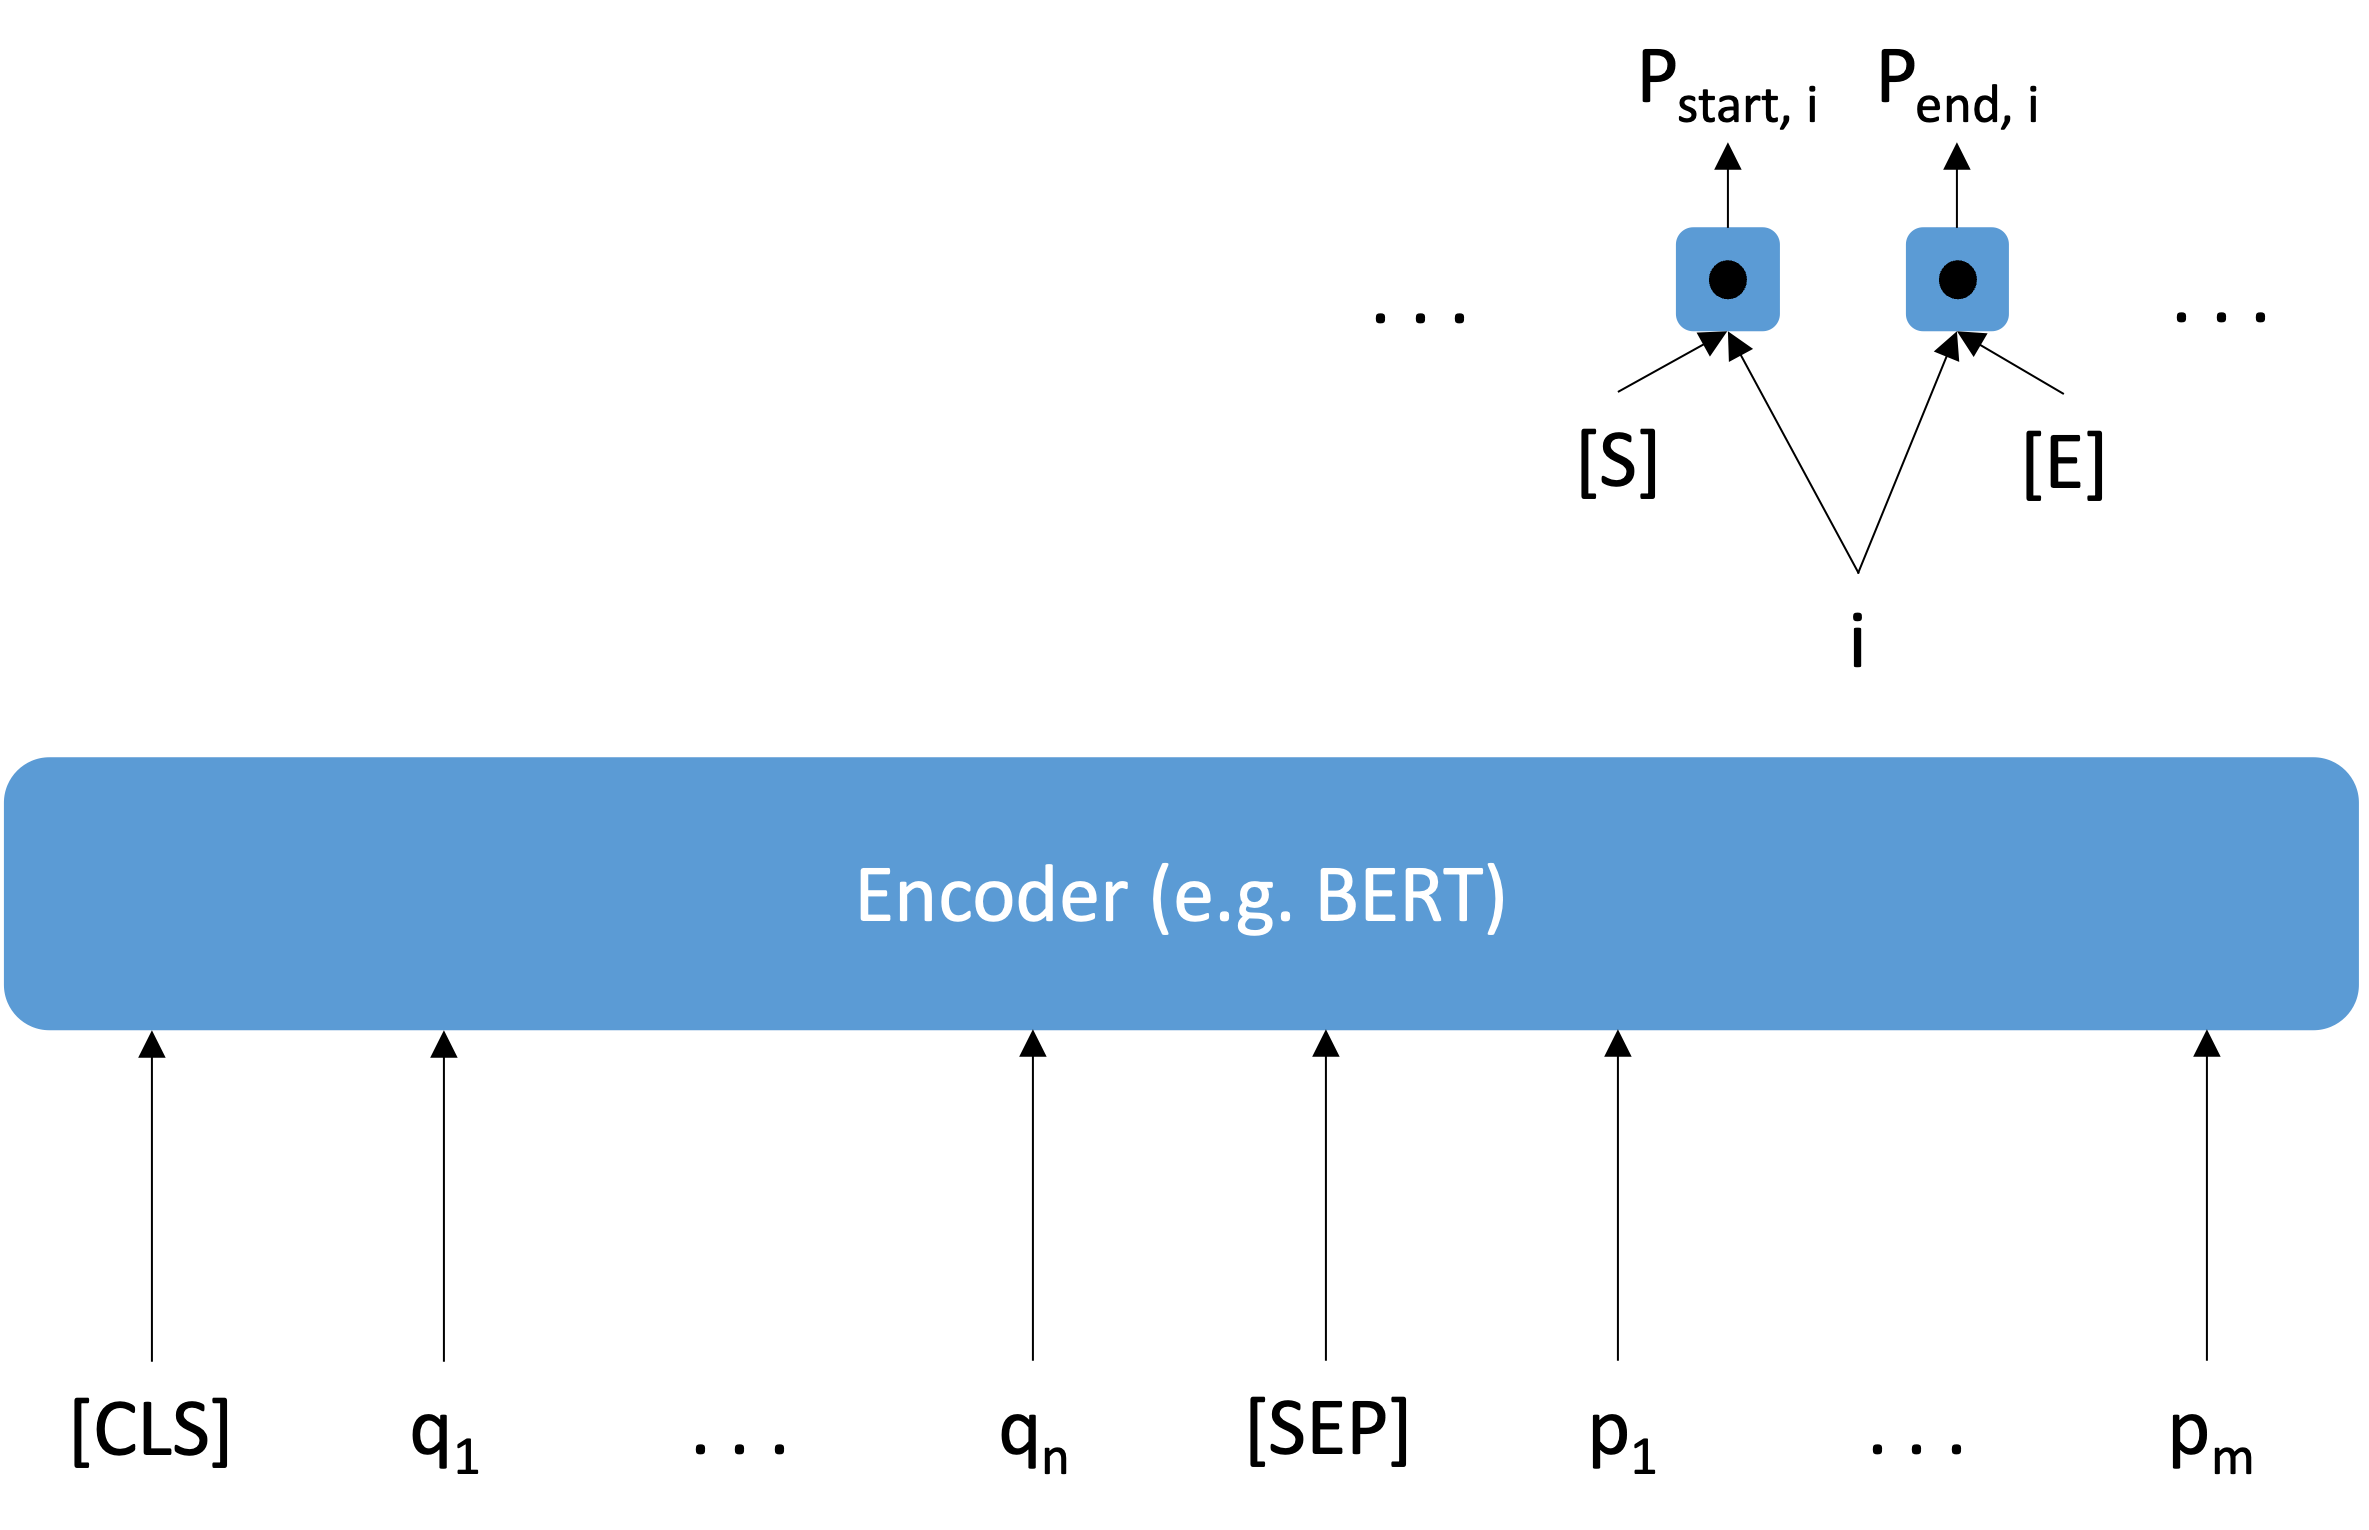
\includegraphics[width=\textwidth]{Grafiken/Extractive_Reader.png}
    \caption{Adjusted Graphic of the Extractive Reader by Jurafsky et al. \cite{jurafsky_speech_2023}}
    \label{fig:extractive_reader}
\end{figure}

The \textbf{Generative Reader} operates straightforwardly when familiar with a \gls{s2s} encoder-decoder model. Given a dataset containing $(q,p,a)$ tuples, the encoder takes $q$ and $p$ as input and outputs the contextual representation $h$. Then, it is the decoder's task to generate a token sequence based on $h$ and attention. The training objective can be described as minimizing the following loss function:

\begin{equation}
    \mathbf{\mathcal{L}_{\mathrm{Gen}}=\sum_{i=1}^K \log \mathbf{P}\left(a_i \mid \mathbf{h}, a_{: i}\right)}
\end{equation}

Here, $K$ represents the length of tokens in $a$, $a_i$ is the $i^{th}$ token in $a$, and $a_0$ is a special beginning of sequence token. In cases where the answer is not contained within the passages, the \verb|[CLS]| token indicates this situation \cite{luo_choose_2022,zhu_retrieving_2021}.

Latest research projects like Visconde \cite{pereira_visconde_2022} even employ \gls{llm} as Generative Readers. The performance and usability of these models remain active topics of research.

Luo et al. conducted the first survey comparing state-of-the-art Extractive and Generative Readers \cite{luo_choose_2022}. They discovered that \enquote{on average, extractive readers perform better than generative ones} \cite{luo_choose_2022}, except in cases involving long context passages, where generative approaches outperform the extractive ones.

The \textbf{Answer Post-Processor} is similar to the Document Post-Processor, serving as an optional component. Its primary task is to provide support for multi-hop complex questions, helping determine the final answer from a set of answers extracted by the reader component \cite{zhu_retrieving_2021}. Depending on the implementation of the Reader, this component may become obsolete.

% Commit #5

\subsection{Limitations}
\label{subsec:qa_limitations}

The evaluation metrics for \gls{ir} systems will be discussed in detail in Section \ref{chap:eval}. In general, selecting the components and models for an \gls{ir} system always involves a trade-off between accuracy, memory consumption, and inference speed \cite{zhang_survey_2023}.

Accuracy is primarily determined by the chosen Retriever-Reader-System. Sparse retrievers often lack a certain degree of semantic understanding, resulting in less accurate retrieved passages. In contrast, Dense Retrievers can achieve higher levels of accuracy but require thorough evaluation and training for the desired use case. Thakur et al. demonstrated that high-accuracy Dense Retrievers like \gls{dpr} can underperform in zero-shot scenarios compared to BM25 by -47.7\% \cite{thakur_beir_2021}. This highlights another crucial limitation of all \gls{nn}-based retrievers and readers: training. BM25 is, by nature, an unsupervised model for \gls{ir}, while common approaches for Dense Retrieval usually belong to the group of supervised models. These models heavily depend on their training data, whereas a Sparse Retriever like BM25 can be used without any training. According to experiments conducted by Thakur et al. \cite{thakur_beir_2021}, the best-performing out-of-distribution Retrievers are Representation-Interaction Retrievers like ColBERT.

Constructing a training dataset for a \gls{qa} task can be a tedious process, as these datasets must consist of tuples in the form of $(\text{question, context, answer})$, which is not always feasible. One established research direction to address this issue is \gls{qg} \cite{serban_generating_2016}. In \gls{qg}, a \gls{s2s} model is employed to generate questions and answers based on a given passage.

Zhang et al. provide an example of \gls{dpr} applied to the Natural Questions dataset in their survey on efficient \gls{odqa} \cite{zhang_survey_2023}. The total processing time for a query is 0.91 seconds\footnote{It's important to mention that \gls{dpr} is a Representation-based Retriever, which allows offline storage of passage embeddings. The result was obtained using an Nvidia GeForce Rtx 2080 Ti GPU, averaged over 1000 examples}. This time is divided into 74.79\% for evidence search and 23.95\% for reading. The total memory cost is 79.32GB, with the index occupying 81.95\%, the raw corpus 16.39\%, and the model 1.66\%. Approaches to optimize this may include:

\begin{enumerate}
    \item Reducing Processing Time: (1) Accelerating Evidence Search, (2) Accelerating Reading
    \item Reducing Memory Cost: (1) Reducing Index Size, (2) Reducing Corpus Size, (3) Reducing Model Size
    \item One-stage Frameworks: (1) Directly Generating Answers, (2) Directly Retrieving Answers
\end{enumerate}

Techniques used in this context may include:

\begin{enumerate}
    \item Data-based: (1) Passage Filtering, (2) Dimension Reduction, (3) Product Quantization
    \item Model-based: (1) Model Pruning, (2) Knowledge Distillation, (3) Knowledge Source 
\end{enumerate}

For a detailed overview of approaches towards more efficient \gls{odqa} systems, please refer to the comprehensive survey by Zhang et al. \cite{zhang_survey_2023}.


\section{Conversational Question Answering}
\label{sec:cqa}

\subsection{Basics}
\label{subsec:cqa_basics}

\subsection{Query Expansion}
\label{subsec:cqa_query_expansion}

\subsection{Initiative}
\label{subsec:cqa_initiative}

\subsection{Large Language Model based Agents / Chain of Thought ???}
\label{subsec:cqa_llm_agents}

\section{Related Work}
\label{sec:related_work}

\subsection{Question Answering based on PDFs}
\label{subsec:related_work_dbqa}

\textbf{PDF Question Answering} is the task of providing answers to questions related to the content of one or multiple documents \cite{mathew_document_2021}. This field of research actively explores the development of an IR-QA system that operates on images of documents. An exemplary architecture and a general pipeline for transforming PDFs into an IR-QA system is presented by McDonald et al. \cite{mcdonald_detect_2022}. They developed their zero-shot framework around the QASPER dataset but used the original PDFs instead of extracted text via LaTeX. Moreover, readily available open-source tools like V-Doc \cite{ding_v-doc_2022} simplify the deployment and testing of datasets, models, and IR-QA systems.

More recently, the open-source framework \textit{Langchain} has gained tremendous attention\footnote{As of September 24, 2023, Langchain has received 63k stars on GitHub}. Langchain focuses on harnessing LLMs using chains, which are essentially prompts for an LLM that can be chained together \cite{noauthor_langchain-ailangchain_nodate}. They also provide documentation on building a QA system based on PDFs \cite{noauthor_question_nodate}. Similarly, \textit{OpenAI} offers a Retrieval Plugin for \textit{ChatGPT} \cite{noauthor_chatgpt_2023}, also an open-source repository. These QA systems adhere to the paradigms established in previous works such as \cite{karpukhin_dense_2020,ni_large_2021,neelakantan_text_2022,lewis_retrieval-augmented_2021}. Specifically, this entails:

\begin{itemize}
    \item Given a text corpus, documents can be retrieved by extracting relevant passages. Data cleaning of the corpus is optional but can be integrated. Therefore, these systems employ a \textit{direct extraction} approach, especially when dealing with PDFs.
    \item Utilizing large-scale, diversely trained encoders. Representation-based Retrievers, when equipped with sufficient trainable parameters and diverse training datasets, often yield comparable results to fine-tuned, more complex retrieval models \cite{ni_large_2021,neelakantan_text_2022}.
    \item Using the LLM as a generative reader for QA, as demonstrated in the work of Izacard et al. \cite{izacard_leveraging_2021}.
\end{itemize}

Non-LLM research for \gls{qa} based on PDFs is notably scarce. In the field of ODQA, discussions regarding applicable frameworks that encompass the entire pipeline from PDFs to \gls{qa} are infrequent. Instead, the focus often revolves around constructing \gls{qa} systems using predefined and well-supervised datasets. However, there is some research that explores the feasibility of deploying high-performing \gls{qa} systems in out-of-domain scenarios, bypassing the initial stage of data preprocessing (from PDFs to passages). This research strives to outline possibilities for using a \gls{qa} system in real-world applications.

\noindent \textbf{Out-of-Domain QA}: As emphasized by Thakur et al. in their \enquote{Heterogeneous Benchmark for Zero-shot Evaluation of Information Retrieval Models} (BEIR) \cite{thakur_beir_2021}, dense retrievers exhibit weak out-of-domain performance. Lyu et al. \cite{farea_evaluation_2022} also demonstrate the limited generality of dense retrievers when trained in one subdomain and subsequently applied in a different one. This underscores the conclusion that there are two approaches to employing retrievers in out-of-domain scenarios: (1) fine-tuning or (2) zero-shot, but with large encoders that have been trained on diverse datasets \cite{ni_large_2021}.

The challenge with fine-tuning lies in the unavailability of labeled data, which is typically required for supervised models in the form of tuples such as $(\text{question, answer, context})$. Several diverse approaches have been developed to address this issue. One approach employs \gls{qg} techniques, as exemplified by Promptagator \cite{dai_promptagator_2022}, which utilizes LLMs. Another strategy involves the use of Mixture-of-Experts and meta-learning algorithms \cite{chen_improving_2021}. Some researchers have explored semi-supervised training datasets, as demonstrated by Sachan et al. \cite{sachan_questions_2023}, who developed ART, a training framework for dense retrievers that only requires questions and surpasses the standard \gls{dpr} training implementation.

Gholami et al. \cite{gholami_zero-shot_2021} experimented with non-fine-tuned dense retrievers on a non-\gls{qa} dataset, specifically a basic collection of AWS documentations. Their results, particularly for the retrieval component, were inconclusive, aligning with the findings of benchmark studies by Thakur et al. \cite{thakur_beir_2021} and Lyu et al. \cite{farea_evaluation_2022}.

On the other hand, there exist reader components with a high degree of generalizability, as demonstrated by UnifiedQA-v2 \cite{khashabi_unifiedqa-v2_2022}, an extractive reader, and T5 \cite{raffel_exploring_2023}, a generative reader.


\subsection{Open-domain Conversational Question Answering ???} 
\label{subsec:related_work_cqa}